\subsection{Håggesund}
\label{haggesund}
%
Håggesund är en hamnstad på sydvästkusten i landet \textit{Norgeria}. Det är i stort sätt självförsörjande, men exporterar lite fisk samt fartyg och båtar från \textit{Bröderna Bågs Båtbyggeri} \sectiondescribe{\ref{brodernaBagsBatbryggeri}}. 
Alla byggnader i Haugesund är byggda i äldre förgrånat trä och är något slitna, likt en gammal nordlig fiskarstad.
%
\begin{figure}
	\centering
	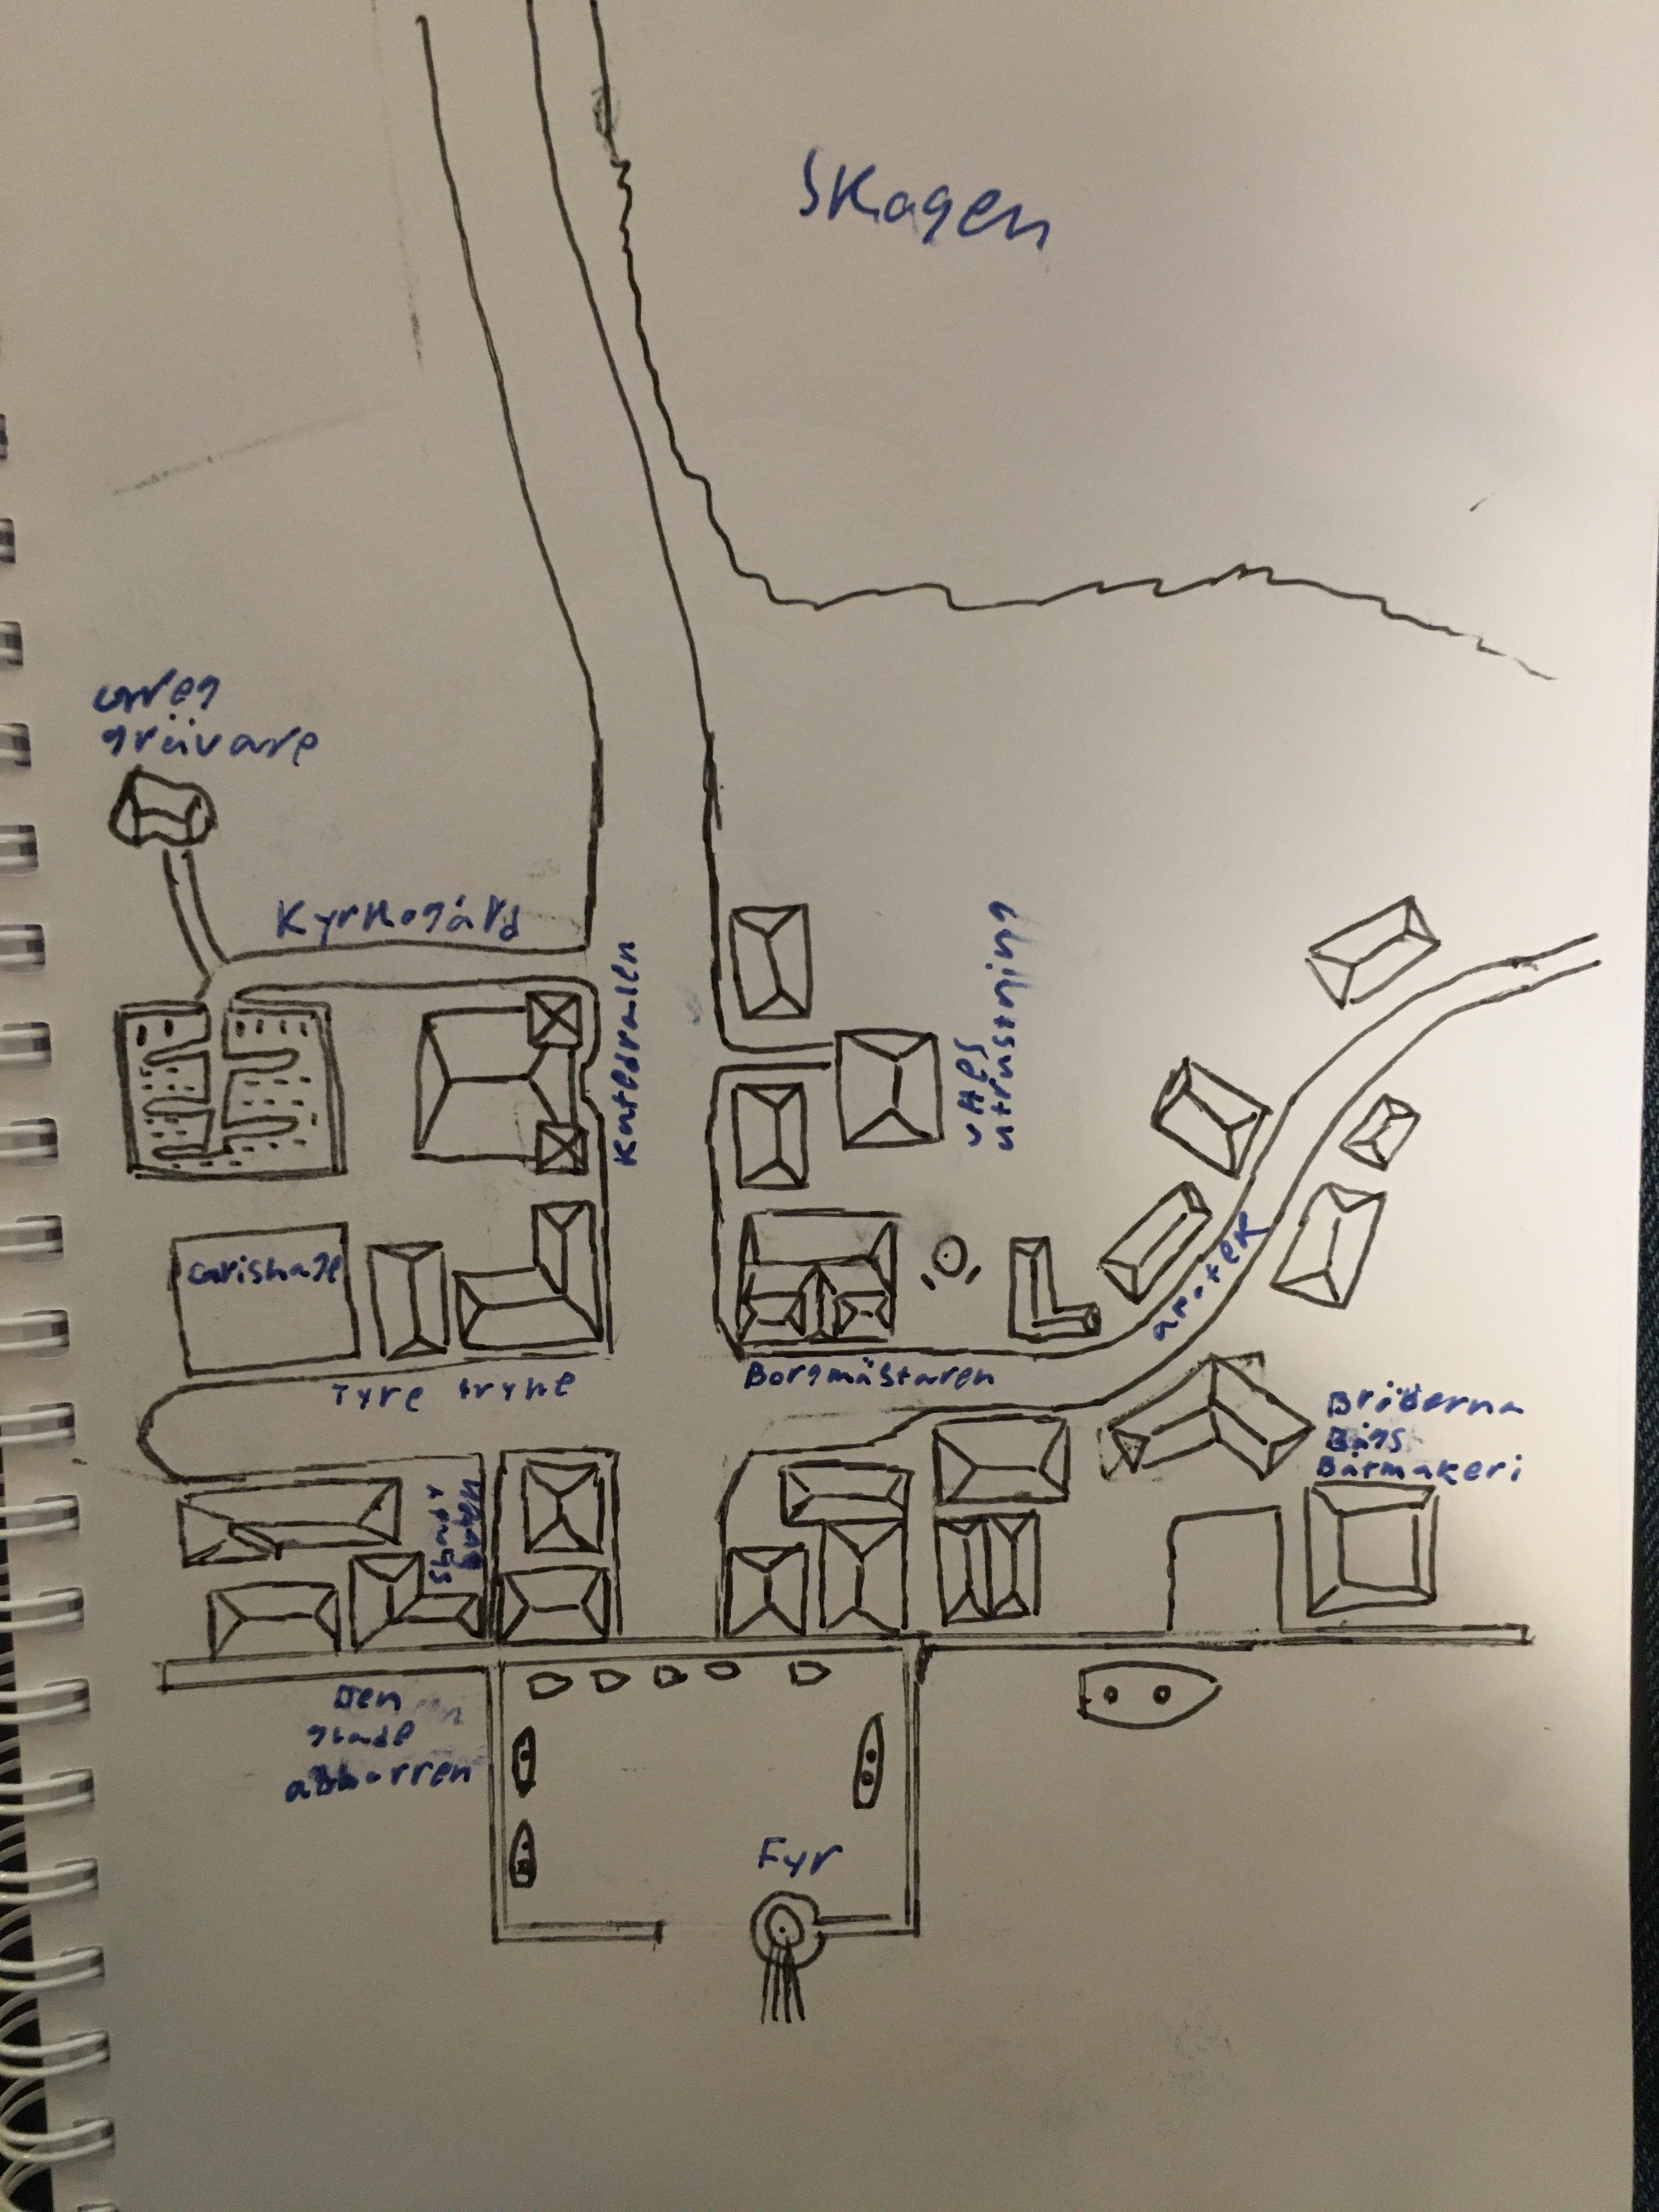
\includegraphics[width=\textwidth]{Haggesund}
	\caption{Håggesund}
\end{figure}
%
\subsubsection{Den glada abborren}
\label{haggesund:denGladaAbborren}
Den glada abborren är ett värdshus som ägs av Oskar, en högljudd kraftig man med flint och ölmage. Det finns utställt stolar och bord i det stora rummet och en bar längst in. I ett av hörnen finns en brinnande eldstad med en grupp fåtöljer. 
%
\paragraph{Mörtmannen Gurgler}
I en av fåtöljerna sitter en Mört-man \sectiondescribe{\ref{mortman}}, Gurgeler, med en huva för att dölja sin ras. Han är inte jättetaggad på att prata med äventyrarna, men kan berätta att han är en köpman från Mehec’ger, 
en by i havet utanför Haugesund. Han har tio guld på sig från handel % TODO: Vad säljer Gurgler?
%
\subsubsection{Borgmästarens hus/Stadshuset}
Borgmästare Korre Upt bor i stadshuset, en av de större byggnaderna i Håggesund. Stadshuset är lågt upplyst och utsmyckat med färglada tyger samt tavlor föreställande Griffins. I den stora salen i mitten av stadshuset sitter Korre Upt i en soffgrupp tillsammans med två andra överviktiga män. Dessa är Korres rådgivare som sitter och röker pipa i varsin soffa.

Korre är en kort liten man med oljigt svart hår samt en lång, tunn mustasch. Korre har en oerhörd fascination av Griffins, och har ett uppdrag angående dessa \sectiondescribe{\ref{korresGriffins}}.
%
\subsubsection{Apoteket}
Apotekare August säljer påfyllning till Medical Kits, Potion of healing och lite grundläggande magiska örter.
%
\subsubsection{Shady Sven}
Shady Sven säljer knark.
% TODO: Utveckla Shady Sven
%
\subsubsection{Tyre Tryne och hans grishage}
% TODO: Skriv om Tyre Trynes grishage. 
Mocka bajs för silvermynt.
%
\subsubsection{Bröderna Bågs Båtmakeri}
\label{brodernaBagsBatbryggeri}
% TODO: Skriv om Bröderna Bågs Båtmakeri
%
\subsubsection{Uffes utrustning}
% TODO: Skriv om uffes utrustning
%
\subsubsection{Katedralen}
Präst
Tillber Den Djupe
Den djupe sägs leva i ett sjunket skepp någonstans i havet långt utanför Haugesund
Där samlar han på skatter som sjunkit till havsbotten
% TODO: Utveckla Katedralen, presten och religionen i Håggesund
%
\subsubsection{Kyrkogård}
% TODO: Skriv nått om kyrkogården
% 
\subsubsection{Greg Gravgrävare}
% TODO: Skriv om Greg Grävare till mer flytande stilP
Gregs hus är liten och väldigt sliten. Där inne är det fullt med bråte och luktar unket. Det finns tre fönster utan gardiner. På fönsterkarmarna står det glasburkar med namn skrivna på och gulvit vätska i som har sjunkit till botten. Det är Gregs säd.

Greg är nekrofil. Han mastruberar till döda kvinnor och sorterar samt lagrar sin säd i burkar med deras namn på. Detta berättar han gärna om och blir exalterad om man frågar om det. Greg skäms inte.

